
%(BEGIN_QUESTION)
% Copyright 2014, Tony R. Kuphaldt, released under the Creative Commons Attribution License (v 1.0)
% This means you may do almost anything with this work of mine, so long as you give me proper credit

This gas incinerator renders streams of toxic gas harmless by high-temperature combustion, oxidizing compounds such as hydrogen sulfide (H$_{2}$S), ammonia (NH$_{3}$), and nitric acid (HNO$_{3}$) to water vapor and other compounds such as sulfur dioxide (SO$_{2}$) that are far less dangerous:

$$\includegraphics[width=15.5cm]{i0004rx01.eps}$$

Stack gas analyzer AT-35 monitors sulfur dioxide gas (SO$_{2}$) emitted into the atmosphere by the incinerator, using optical fluorescence.  Supposing the high-voltage power supply for the photomultiplier tube inside of AT-35 fails to zero volts output, describe the effect this will have on the signal output by AT-35.  Will it register low SO$_{2}$ concentration, high SO$_{2}$ concentration, or will there be no effect on AT-35's output signal?

\vskip 10pt

Supposing thermocouple TE-37 fails shorted at the terminal block where the extension wires connect, what effect will this have on the incinerator's effectiveness in oxidizing harmful compounds?  Will this fault create a condtion where toxic gases could pass through the incinerator unoxidized?

\vskip 10pt

Suppose the chemical composition of fuel gas changes such that it now possesses a greater density ($\rho$) as well as a greater specific heat ($c$), will flow transmitter FT-38 register falsely high, falsely low, or continue to register accurately?

\underbar{file i00964}
%(END_QUESTION)





%(BEGIN_ANSWER)

4 points for correct AT-35 answer, 3 points for correct TE-37 answer, and 3 points for correct FT-38 answer.

\vskip 10pt

If the HV power supply in AT-35 fails with a low output, the photomultiplier tube will stop working and the analyzer will not register any SO$_{2}$ at all because it will not be able to ``see'' the fluorescence of SO$_{2}$ gas.
 
\vskip 10pt

If TE-37 fails shorted at the terminal block it will cause TT-37 to register ambient temperature, causing the fire control system to ramp up fuel flow and make a hotter fire.  This will {\it not} pose a hazard for toxic gas emissions as a lack of flame would.

\vskip 10pt

If the chemical composition of fuel gas changes, FT-38 will continue to register accurately because it is a Coriolis true-mass flowmeter.

%(END_ANSWER)





%(BEGIN_NOTES)

{\bf This question is intended for exams only and not worksheets!}.

%(END_NOTES)


